%% PGCT 연구 진행 논문형 보고서 (2026-10-23). Overleaf: Compiler = pdfLaTeX (한글 글꼴 오류가 나면 XeLaTeX).
%% 그림은 figures/ (make_figures.py로 생성, 학습 없음).
\documentclass[10pt]{article}
\usepackage[a4paper,margin=2.3cm]{geometry}
\usepackage{kotex}
\usepackage{amsmath,amssymb,amsthm}
\usepackage{graphicx}
\usepackage{booktabs}
\usepackage{tabularx}
\usepackage{xltabular}
\usepackage{array}
\usepackage{enumitem}
\usepackage{placeins}
\usepackage[small]{caption}
\usepackage[hidelinks,unicode]{hyperref}

\newtheorem{proposition}{명제}
\newtheorem{assumption}{가정}
\newtheorem{definition}{정의}
\newcommand{\JS}{\operatorname{JS}}
\newcommand{\KL}{\operatorname{KL}}
\newcommand{\sg}{\operatorname{sg}}
\newcolumntype{L}{>{\raggedright\arraybackslash}X}
\newcommand{\easy}[1]{\par\smallskip\noindent\fbox{\parbox{\dimexpr\linewidth-2\fboxsep-2\fboxrule}{\small\textbf{쉽게 말하면.} #1}}\par\smallskip}
\newcommand{\detail}[1]{\par\smallskip\noindent\fbox{\parbox{\dimexpr\linewidth-2\fboxsep-2\fboxrule}{\small\textbf{자세히 보면.}\begin{itemize}[leftmargin=1.2em,itemsep=0pt,topsep=2pt]#1\end{itemize}}}\par\smallskip}
\setlist{itemsep=1pt,topsep=3pt}
\renewcommand{\arraystretch}{1.12}

\title{Probe-Gated Critic Transfer:\\ 잠재 팀 발견과 선택적 critic 전이\\[4pt] \large 연구 진행 보고 --- 기존 실험, 진행 중인 실험, 향후 계획}
\author{이환률}
\date{2026년 10월 23일}

\begin{document}
\maketitle

\begin{abstract}
여러 팀이 한 공간을 공유하는 다중 agent 강화학습에서, agent는 이웃 가운데 누가 같은 목표를 가진 팀원인지 모를 수 있다.
Probe-Gated Critic Transfer(PGCT)는 모든 agent가 같은 probe 관측에 대한 행동 분포를 비교해 팀원을 추정하고, 추정된 팀원의 critic만 증류하는 완전 분산 방법이다.
지금까지의 실험에서 행동 분포 전체를 JS로 비교하는 정책 probe는 어느 설정에서도 팀을 안정적으로 가르지 못했다(팀 AUROC 0.41--0.78).
그러나 지도에서 계산한 ``goal 방향 축''으로 정책 응답을 투영하면, 6-agent 칸에서 agent의 goal 쪽이 0.89--0.96의 AUROC로 드러났고, 단순한 부호 규칙이 팀 쌍의 76--83\%를 맞혔다. 보상 결합이 실패하는 개인 보상 칸도 포함된다.
원인을 추적하면서 환경의 문제도 드러났다. 선반 집기 감점 때문에 학습 초기 0.1--0.2M step에 모든 agent가 선반 집기를 포기했고, 결과가 ``누가 먼저 재발견하나''라는 운에 좌우되었다.
감점을 .02에서 .005로 낮추자 1M 시점 배송이 5배 이상 늘었지만, 여전히 한 agent가 배송의 82--99\%를 맡았다.
팀 보상 환경에서는 ``남의 배송이 내 보상을 바꾸는가''를 묻는 보상 결합 probe가 팀을 완벽히 갈랐고(AUROC 1.00), 대개 1--4만 step 안에 모든 쌍을 식별했다.
이에 따라 연구 목표는 유지하되, 기여를 ``어떤 조건에서 국소 신호로 잠재 팀을 찾을 수 있는가''로 재정의하고, 같은 기반 위의 2$\times$2 설계로 검증한다.
현재 팀원 critic 전이의 효용을 5M step, seed 3개로 시험하고 있다.
\end{abstract}

\tableofcontents

%% ==================================================================
\section{서론}

두 회사의 로봇이 한 창고를 공유한다고 하자. 각 로봇은 자기 회사가 요청한 선반을 자기 회사의 배송 지점으로 옮긴다.
협력형 MARL에서는 목표가 같은 agent끼리 파라미터·경험·가치 추정을 나누면 표본 효율이 좋아진다 \cite{christianos2020,christianos2021}.
그러나 목표가 다른 agent의 critic을 배우면 다른 목표의 가치 쪽으로 편향될 수 있다.
팀원이 누구인지는 항상 주어지지 않는다. 공통 식별 체계가 없을 수 있고, 배치마다 팀 구성이 달라질 수 있다.

본 연구는 세 질문을 구분한다.
\begin{itemize}
  \item \textbf{Q1 (식별)}: agent는 국소 정보만으로 이웃 가운데 팀원을 찾을 수 있는가?
  \item \textbf{Q2 (전이 효용)}: 팀을 정확히 알고 critic을 공유하면 학습에 실제로 도움이 되는가?
  \item \textbf{Q3 (선택적 전이)}: 잘못된 상대를 배제하는 것이 무차별 공유보다 나은가?
\end{itemize}

\paragraph{현재까지의 결론.}
(1) 행동 분포 전체의 JS로 비교하는 정책 probe는 팀을 가르지 못했다.
(2) 같은 정책 응답을 ``goal 방향 축''으로 투영하면 팀 차이가 드러난다. 개인 보상 칸에서도 부호 규칙이 팀 쌍의 83\%를 맞혔다(\ref{sec:axis}절).
(3) 팀 보상이 있으면 보상 결합 probe로 팀을 빠르고 정확하게 찾는다. 다만 이 신호는 사실상 팀의 정의에 가까워, 방법으로서의 새로움은 제한적이다.
(4) Q2는 Oracle-team 대 IPPO 비교(5M, seed 3개)로 시험 중이다.

\begin{table}[h]
\centering
\caption{결과 한눈에 보기. 각 실험이 무엇을 물었고, 한 줄로 무엇을 알았는지.}
\label{tab:glance}
\begin{tabularx}{\textwidth}{>{\raggedright\arraybackslash}p{3.4cm} L >{\raggedright\arraybackslash}p{1.4cm}}
\toprule
실험 & 한 줄 결론 & 절 \\
\midrule
E1 (6.4M, seed 1) & PGCT가 빨라 보였지만 gate는 팀원을 고르지 못했다. seed 하나라 운일 수 있다. & \ref{sec:e1} \\
probe 점검, 보상 probe $\hat r$ & 행동 JS도, ``내 행동의 예측 보상''도 팀을 믿을 만하게 가르지 못했다. & \ref{sec:probecheck} \\
E1-F, 후보 A·B & 목표를 갈라도, 팀 보상을 줘도 2M 안에 한 agent만 배웠다. & \ref{sec:e1f} \\
선반 집기 정체 & 학습 초기에 선반 집기가 가장 손해라서 모두가 0.1--0.2M에 포기했다. 원인은 감점이었다. & \ref{sec:stall} \\
감점 .005 (1M) & 배송이 5배 이상 늘었지만, 여전히 한 agent가 대부분을 배송한다(1M 시점). & \ref{sec:pen005} \\
보상 결합 probe & 팀 보상이면 팀을 완벽히 가르고(AUROC 1.00) 1--4만 step 안에 다 찾는다. 개인 보상이면 실패한다. & \ref{sec:ident} \\
goal 방향 축 & 정책 응답을 ``왼쪽 goal 행동 대 오른쪽 goal 행동''으로 보면, 개인 보상 칸에서도 팀이 상당히 갈린다. & \ref{sec:axis} \\
독주 진단 & 독주 agent를 빼도 나머지는 배송하지 않는다. 밀려난 게 아니라 아직 못 배운 것이다. & \ref{sec:pen005}, \ref{sec:limits} \\
\bottomrule
\end{tabularx}
\end{table}

\paragraph{기여(현재 구도).}
연구 목표(잠재 팀 발견 + 팀 내 critic 전이)는 유지한다.
기여는 gate 메커니즘 자체가 아니라, 어떤 팀 구조에서 어떤 국소 신호로 팀을 식별할 수 있는지에 대한 조건(4절)과, 조건에 맞춘 두 종류의 probe(행동 probe, 보상 결합 probe)다.

%% ==================================================================
\section{관련 연구}

\paragraph{같은 목표 이웃과의 공유.}
Du et al.\ \cite{du2025}은 분산 환경에서 agent가 관측 범위 안의 이웃과 목표를 명시적으로 교환하고, 같은 목표를 가진 이웃과만 actor·critic 가중치를 평균한다. 본 연구의 Oracle-team은 사실상 이 방식의 critic 전용판이다. PGCT의 차이는 목표나 팀 라벨을 교환하지 않는다는 점이다.

\paragraph{학습 상대의 선택.}
Peer Learning \cite{derstroff2024}은 누구의 조언을 따를지를 bandit 문제로 다루며, 측정된 유용성으로 상대를 고른다. PGCT는 유용성이 아니라 팀 관계를 추정 대상으로 둔다.
SEAC \cite{christianos2020}는 다른 agent의 경험이 자신에게도 유익하다는 가정 아래 경험을 공유하며, RWARE를 제안한 연구이기도 하다. PGCT의 동기는 이 가정이 깨질 수 있는 잠재 다중 팀 환경이다.

\paragraph{선택적·동적 공유.}
SePS \cite{christianos2021}는 학습 전에 agent를 군집화해 군집 안에서 파라미터를 공유하고, MADPS \cite{hu2024}는 정책 거리를 재어 공유를 조절한다. PGCT는 중앙 군집화 없이 현재 이웃 가운데서 국소적으로 상대를 고른다.

\paragraph{행동으로 정체 추론.}
IDRL \cite{idrl}은 hidden-role 게임에서 관계 네트워크로 다른 agent의 정체를 추론하지만, 그 결과를 정책 선택에 쓴다. 본 연구는 추론 결과를 critic 전이 대상 선택에만 쓴다.

\paragraph{분산 critic과 증류.}
networked actor-critic \cite{zhang2018}은 공통 평균 목표 아래 이웃과 critic을 평균한다. 본 연구의 critic은 비선형이고 보상이 팀마다 다르므로 그 보장이 그대로 적용되지 않는다. PGCT는 파라미터 평균 대신 probe 입력에서의 출력 증류 \cite{rusu2016}를 쓴다.

%% ==================================================================
\section{문제 설정}

agent $i \in \{1,\dots,N\}$로 이루어진 부분 관측 확률 게임을 생각한다. 각 agent는 팀 $z_i \in \{1,\dots,K\}$에 속하며, 팀은 어떤 선반이 요청되는지와 어디로 배송하는지를 정한다.
관측은 자기 팀에 필요한 정보를 담지만 다른 agent의 팀 $z_j$는 담지 않는다. 통신 범위 안의 agent가 이웃 $\mathcal{N}_i(t)$이다.
이웃끼리는 probe 입력에 대한 네트워크 출력만 교환하며, 관측·보상·파라미터·팀 라벨은 교환하지 않는다.
각 agent는 순환 actor $\pi_i$와 critic $V_i$를 PPO \cite{schulman2017}로 학습한다.

\begin{definition}[부분 팀 관계]
$\mathcal{T}_i(t) = \{ j \in \mathcal{N}_i(t) : z_j = z_i \}$. 모든 $i$에서 추정 $\hat{\mathcal{T}}_i(t) = \mathcal{T}_i(t)$이면, 그 방법이 시점 $t$에서 부분 팀 관계를 복원한다고 한다.
\end{definition}

%% ==================================================================
\section{방법}

\begin{figure}[t]
  \centering
  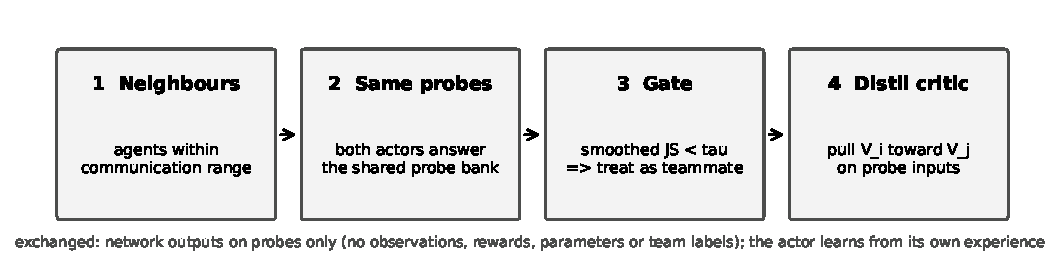
\includegraphics[width=\textwidth]{figures/fig_overview.pdf}
  \caption{PGCT의 네 단계. 통신 범위 안의 이웃끼리 같은 probe에 대한 행동 분포를 비교하고, 평활한 JS divergence가 임계값보다 작은 이웃을 팀원으로 보아 그 critic을 증류한다.}
  \label{fig:overview}
\end{figure}

\subsection{Probe 집합}
probe는 작고 통제된 상황 하나를 나타내는 관측이다. 모든 probe는 학습 전에 지도에서 정해진 규칙으로 만들어지므로, 모든 agent가 통신 없이 같은 집합을 갖는다.
probe는 순환 상태를 0으로 두고 action mask 없이 평가한다.

\begin{assumption}[probe 비교 가능성]
모든 probe는 모든 agent에게 유효한 관측이며, 관측하는 agent 자신의 목표에 대한 상황을 모두에게 같은 방식으로 나타낸다.
\end{assumption}

probe는 두 역할을 한다. gate 집합 $\mathcal{Q}_{\mathrm{gate}}$에는 팀에 따라 최적 행동이 달라지는 상황(예: 운반 중이고 goal이 보이지 않음)이 필요하다. 증류 집합 $\mathcal{Q}_{\mathrm{dist}}$에는 과제의 모든 단계를 덮는 넓은 범위가 필요하다(그림 \ref{fig:probes} 위 두 줄).
canonical 설정은 두 역할에 같은 48개를 쓰고(서로 다른 입력 26개), v2 설정은 gate 48개와 증류 64개를 따로 쓴다.

\subsection{응답 비교와 gate}
$p_i^m = \pi_i(\cdot \mid q_m, h = 0)$이라 하자. 이웃은 $P$ update마다 응답을 교환해
\[
  D_{ij} = \frac{1}{M}\sum_{m=1}^{M} \JS(p_i^m, p_j^m), \qquad
  \JS(p,q) = \tfrac12 \KL(p \,\|\, \bar p) + \tfrac12 \KL(q \,\|\, \bar p),\ \bar p = \tfrac{p+q}{2}
\]
를 계산하고, $\bar D_{ij} \leftarrow (1-\beta)\bar D_{ij} + \beta D_{ij}$로 평활한다. warm-up $U_0$ update 뒤 팀원을
\[
  \hat{\mathcal{T}}_i(t) = \{ j \in \mathcal{N}_i(t) : n_{ij} \ge n_{\min},\ \bar D_{ij} < \tau \}
\]
로 추정한다. 설정값은 $P = 5$, $\beta = 0.35$, $\tau = 0.12$, $U_0 = 100$, $n_{\min} = 8$이다.

\subsection{Critic 증류}
\[
  \mathcal{L}_i = \mathcal{L}^{\mathrm{PPO}}_i + \lambda \sum_{j \in \hat{\mathcal{T}}_i(t)} \frac{1}{|\hat{\mathcal{T}}_i(t)|}
  \frac{1}{M_d}\sum_{m=1}^{M_d} \Big( V_i(q^d_m) - \sg\big[V_j(q^d_m)\big] \Big)^2, \qquad \lambda = 0.01.
\]
$\hat{\mathcal{T}}_i$가 비면 peer 항이 사라지고 독립 PPO와 같다. actor는 자기 경험으로만 학습한다.

\subsection{보상 결합 probe}
\label{sec:coupling}
gate 신호만 바꾼 변형이다. 지도에서 공통 사건 집합 $\mathcal{E}$를 정한다(지금은 goal 칸 $g$마다 ``칸 $g$에서 배송이 일어남'' 하나씩).
agent $i$가 시점 $t$에 사건 $e$를 ``봤다''($o_i(e,t)$)는 것은, 남이 일으킨 사건이 자기 시야 안에서 일어났고 그 step에 자신은 배송·반납을 하지 않았다는 뜻이다.
\[
  \rho_i(e) = \frac{\sum_t \mathbb{1}[o_i(e,t)]\, r_i(t)}{\sum_t \mathbb{1}[o_i(e,t)]} - b_i, \qquad
  D^r_{ij} = \frac{1}{|\mathcal{M}_{ij}|}\sum_{e \in \mathcal{M}_{ij}} |\rho_i(e) - \rho_j(e)|,
\]
여기서 $b_i$는 사건이 없던 step의 평균 보상, $\mathcal{M}_{ij}$는 두 agent가 모두 $K$번 이상 본 사건이다. $D^r_{ij} < R/2$($R$: 배송 보상)이면 팀원으로 판정한다.
시뮬레이션이나 신경망 학습 없이 자기 경험의 평균만 쓰며, 보상 자체는 교환하지 않는다. 반응이 모두 0 근처인 경우(개인 보상)에는 판정을 보류하는 규칙이 필요하다(\ref{sec:ident}절).

\subsection{goal 방향 축 통계 (정책 probe의 변형)}
\label{sec:axis-method}
JS는 다섯 행동 전체의 차이를 더한다. 그런데 팀 차이는 ``어느 쪽 goal로 향하는 행동을 고르나''에만 있다. 그래서 그 차이만 뽑아 비교한다.
gate probe 가운데, 지도에서 계산한 최단 경로의 첫 행동이 왼쪽 goal($L_m$)과 오른쪽 goal($R_m$)에서 겹치지 않는 probe 집합을 $\mathcal{Q}^{*}$라 하자(모서리 배치에서 48개 중 13개).
\[
  s_i = \frac{1}{|\mathcal{Q}^{*}|}\sum_{m \in \mathcal{Q}^{*}} \Big( p_i^m(L_m) - p_i^m(R_m) \Big),
\]
$s_i > 0$이면 왼쪽 goal agent처럼, $s_i < 0$이면 오른쪽 goal agent처럼 행동한다는 뜻이다.
두 이웃은 $s_i$만 교환하고, 부호가 같으면 팀원으로 본다(부호 규칙). $|s_i - s_j|$를 거리로 쓸 수도 있다.
팀 라벨과 goal 배정은 쓰지 않는다. 대신 goal 후보 칸이 지도의 어디인지는 안다고 가정한다. 팀이 셋 이상이면 goal 쌍마다 축이 필요하다.

%% ==================================================================
\section{이론}

\paragraph{분리 마진.} $\delta_{\mathrm{in}}(n) = \max_{z_i = z_j} D_{ij}(n)$, $\delta_{\mathrm{out}}(n) = \min_{z_i \ne z_j} D_{ij}(n)$, $\Delta(n) = \delta_{\mathrm{out}}(n) - \delta_{\mathrm{in}}(n)$.

\begin{proposition}[정확한 부분 복원]
$\Delta(n) > 0$, 모든 이웃 쌍에서 $|\bar D_{ij}(n) - D_{ij}(n)| \le \epsilon$, $2\epsilon < \Delta(n)$, warm-up과 $n_{\min}$ 충족, $\delta_{\mathrm{in}} + \epsilon < \tau < \delta_{\mathrm{out}} - \epsilon$이면 모든 $i$에서 $\hat{\mathcal{T}}_i(n) = \mathcal{T}_i(n)$이다.
\end{proposition}

\begin{proposition}[추적 오차]
$|D_{ij}(n) - D_{ij}(n-1)| \le \rho$이면 $|\bar D_{ij}(n) - D_{ij}(n)| \le \frac{1-\beta}{\beta}\rho$이다($\beta = 0.35$에서 계수 1.86).
\end{proposition}

\begin{proposition}[같은 결정 문제를 푸는 팀]
다른 agent의 정책을 고정했을 때 다른 팀 agent의 결정 문제가 관측 좌표에서 같으면, 한 팀에 최적인 기억 없는 사상은 다른 팀에도 최적이다. 최적 사상이 유일하면 모든 쌍에서 $D_{ij} = 0$이고 어떤 임계값도 팀을 가르지 못한다.
\end{proposition}

\paragraph{식별 가능성의 두 원천.}
명제 3의 논리는 비교하는 양이 관측자 기준 $(o,a)$의 함수이면 정책·가치·보상 예측기 모두에 성립한다. 팀을 가를 수 있는 원천은 두 가지다.
\begin{itemize}
  \item (가) \textbf{목표의 기하}: 공통 좌표에서 팀마다 목표 위치가 다르면 행동·가치 probe로 가를 수 있다.
  \item (나) \textbf{보상의 결합}: 남의 사건이 내 보상을 바꾸면(팀 보상) 보상 결합 probe로 가를 수 있다.
\end{itemize}
행동 유사성은 같은 팀의 필요조건도 충분조건도 아니다. 관측이 ``내 기지, 내 자원'' 기준이면 다른 팀의 일꾼도 똑같이 행동하고, 같은 팀이라도 역할을 나누면 다르게 행동한다.

\paragraph{보상 결합의 분리 조건(스케치).}
팀 보상에서 $\rho_i(e_g) \approx R \cdot \mathbb{1}[g \in G_{z_i}]$이다. 추정 오차가 $\epsilon$ 이하이면 같은 팀 쌍은 $|\rho_i - \rho_j| \le 2\epsilon$, goal 칸이 팀마다 하나일 때 다른 팀 쌍은 $|\rho_i - \rho_j| \ge R - 2\epsilon$이다. 따라서 $\epsilon < R/4$이면 $\theta = R/2$가 두 팀을 정확히 가른다(정식 증명은 아님).
개인 보상이거나 두 팀이 goal 칸을 공유하면 이 조건이 깨진다.

%% ==================================================================
\section{환경과 실험 설계}

\subsection{두 팀 RWARE}
다중 로봇 창고(RWARE) \cite{papoudakis2021}의 두 팀 변형을 쓴다. 지도는 11$\times$10 격자에 선반 32개가 있다.
agent는 11$\times$11 시야(센서 범위 5)를 13개 채널로 보고, 절대 위치·방향·적재 상태 등 20개 정보를 함께 받는다.
채널은 팀 기준이다. 자기 팀 요청 선반과 자기 goal이 전용 채널에 표시되며, 다른 agent의 팀은 보이지 않는다.
보상은 배송 +1, 반납 +1, 요청 선반 적재 +0.15와 작은 shaping 항이다. episode는 500 step이다.

\subsection{배치의 변천}
\begin{itemize}
  \item \textbf{E1}: 4 agent, 개인 보상, goal 인접((4,10)/(5,10)), 통신 5, 감점 .02. 두 팀이 거의 같은 문제를 푸는 대칭 조건이다.
  \item \textbf{E1-F}: E1에서 goal만 양쪽 모서리((0,10)/(9,10))로 옮긴 주 실험이었다.
  \item \textbf{후보 A·B}: 팀 보상. A는 4 agent·통신 5, B는 6 agent(3+3)·통신 3이다.
  \item \textbf{2$\times$2 (현재)}: B를 기반으로 감점을 .005로 고정하고, goal 배치(인접/모서리) $\times$ 보상(개인/팀)만 바꾼다(그림 \ref{fig:env}). 설정 대조에서 다른 값은 \texttt{team\_reward\_mode}와 \texttt{team\_goal\_positions}뿐이었다.
\end{itemize}

\begin{figure}[t]
  \centering
  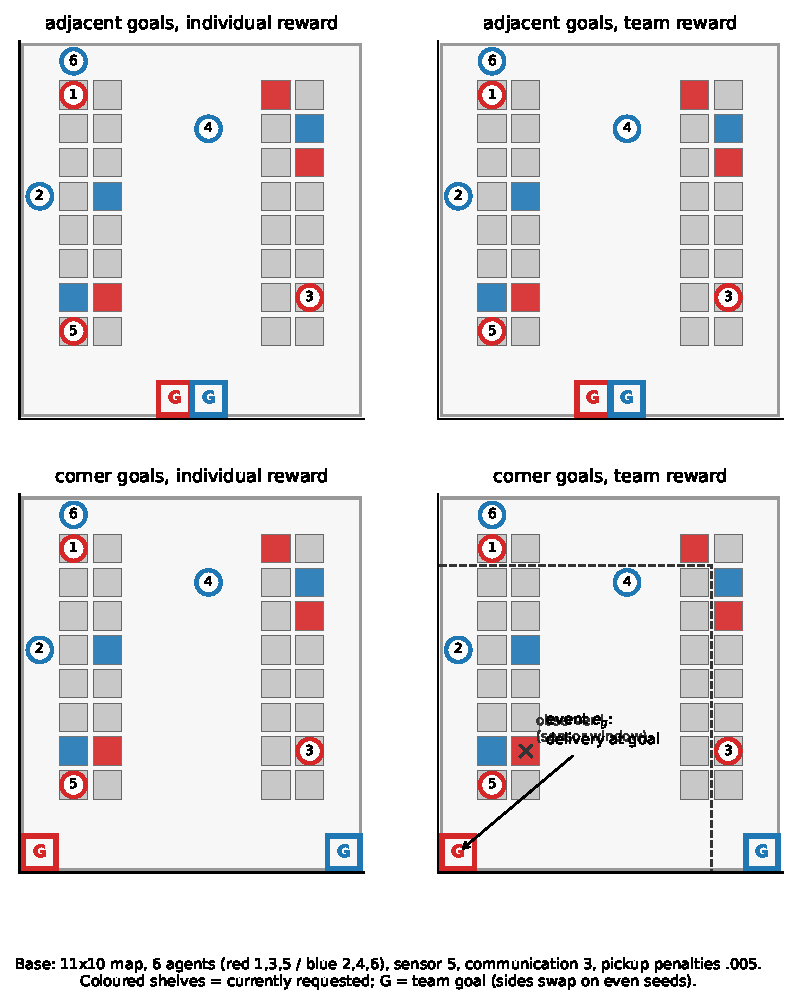
\includegraphics[width=0.78\textwidth]{figures/fig_env_2x2.pdf}
  \caption{같은 기반 위의 2$\times$2 설계(reset seed 5000001). 오른쪽 아래(모서리·팀)에는 보상 결합 probe가 쓰는 공통 사건(goal에서의 배송)과 관측 agent의 시야를 표시했다.}
  \label{fig:env}
\end{figure}

\subsection{비교 방법}
모든 방법은 같은 순환 PPO 학습기(semantic CNN 인코더, 128 unit GRU)와 같은 하이퍼파라미터를 쓰며, seed가 같으면 초기 가중치가 비트 단위로 같다.
\begin{itemize}
  \item \textbf{IPPO}: 전이 없음.
  \item \textbf{All-peer}: 모든 이웃을 donor로 쓴다.
  \item \textbf{Oracle-team}: 실제 팀원만 쓴다(특권 정보를 쓰는 참조 기준).
  \item \textbf{Wrong-team}: 다른 팀 이웃만 쓴다(구현됨).
  \item \textbf{Random-gated}: PGCT가 실제로 만든 연결 수만큼 무작위 이웃을 쓴다(구현됨, smoke까지).
  \item \textbf{PGCT-정책 / PGCT-reward}: 정책 probe gate / 보상 결합 gate(후자는 구현 예정).
\end{itemize}

\subsection{지표}
학습 지표는 결정적 평가(20 episode, 500 step)의 배송 수, 배송을 배운 agent 수, 팀별 배송이다.
식별 지표는 팀 AUROC(같은 팀 쌍이 다른 팀 쌍보다 더 가깝다고 나올 확률)와 온라인 판정의 정답·오답 쌍 수다.

%% ==================================================================
\section{지금까지의 실험}

\subsection{E1: 처음부터 학습 비교 (seed 1, 6.4M)}
\label{sec:e1}

\begin{table}[h]
\centering
\caption{E1 결과(seed 1개, pilot). 시작: 3점 이동평균이 배송 1회(20회)에 처음 도달한 시점. 최종: 마지막 평가 5회 평균 $\pm$ 표준편차.}
\label{tab:e1}
\begin{tabular}{lccccc}
\toprule
방법 & 시작 $\ge 1$ (M) & 시작 $\ge 20$ (M) & 평균 0--6.4M & 최종 & 학습 agent \\
\midrule
IPPO & 2.05 & 5.07 & 10.4 & 23.2 $\pm$ 1.1 & 2/4 \\
All-peer & 3.99 & -- & 3.7 & 19.4 $\pm$ 1.6 & 4/4 \\
PGCT & 1.79 & 4.15 & 11.7 & 27.3 $\pm$ 1.4 & 3/4 \\
Oracle-team & 1.64 & 4.66 & 13.2 & 32.2 $\pm$ 1.7 & 3/4 \\
\bottomrule
\end{tabular}
\end{table}

PGCT가 IPPO보다 빨라 보였지만 gate는 팀원을 고르지 못했다. E1 checkpoint에서 같은 팀 probe 거리는 0.333, 다른 팀은 0.276으로 반대였고(그림 \ref{fig:e1}), 2M 이후에는 팀원 간 전이가 거의 사라졌다.
같은 seed에서도 첫 배송 시점이 0.2--2.1M으로 흔들려, seed 하나의 성능 차이는 운일 수 있다.
\easy{PGCT 점수가 좋게 나왔지만, PGCT가 하려던 일(팀원 고르기)은 하지 못했다. 그래서 점수 차이를 PGCT 덕분이라고 말할 수 없다.}
\detail{
  \item \textbf{조건}: E1(4 agent, 개인 보상, goal 인접 (4,10)/(5,10), 통신 5, 감점 .02), 처음부터 학습, seed 1, 공통 구간 6.4M. 평가는 51,200 step마다 결정적 정책 20 episode $\times$ 500 step.
  \item \textbf{성능}: 배송 1회 도달 시점 IPPO 2.05M, All-peer 3.99M, PGCT 1.79M, Oracle-team 1.64M. 0--6.4M 평균 배송 10.4 / 3.7 / 11.7 / 13.2. 마지막 5회 평균 23.2 / 19.4 / 27.3 / 32.2. 배운 agent 2/4, 4/4, 3/4, 3/4.
  \item \textbf{gate}: checkpoint 진단에서 같은 팀 평균 probe 거리 0.333, 다른 팀 0.276(신호 반전). 2M 이후 PGCT의 팀원 간 연결은 거의 없고 다른 팀 쌍의 산발적 연결만 남았다.
  \item \textbf{재현성}: 같은 seed라도 전이 방법의 첫 배송 시점이 0.2--2.1M 사이에서 흔들렸다(D45).
  \item \textbf{한계}: seed 1개, 방법 간 차이는 episode당 배송 몇 회 수준. E1은 두 팀이 거의 같은 문제를 푸는 대칭 배치다.
  \item \textbf{근거}: EXPERIMENTS E24·E27, \texttt{output/paper\_e1\_20261018/numbers.json}.
}

\begin{figure}[t]
  \centering
  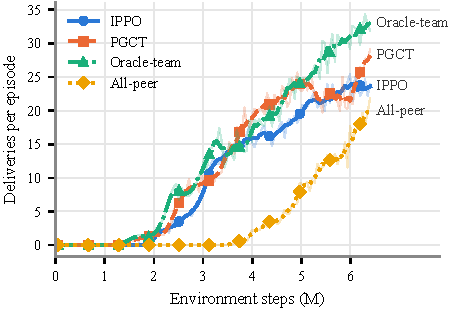
\includegraphics[width=0.48\textwidth]{figures/e1_fig1_learning_curves.pdf}\hfill
  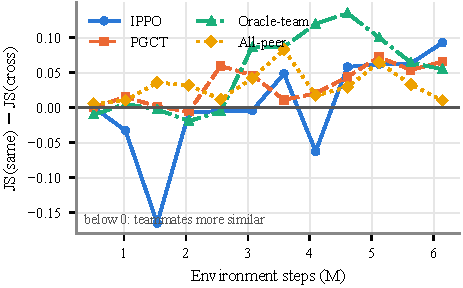
\includegraphics[width=0.48\textwidth]{figures/e1_fig4_probe_js_gap.pdf}
  \caption{E1(seed 1). 왼쪽: 평가 배송. 오른쪽: 팀원 간 평균 probe divergence $-$ 다른 팀 간 평균. 0보다 크면 팀원 응답이 덜 비슷하다는 뜻이다.}
  \label{fig:e1}
\end{figure}

\subsection{Probe 점검과 보상 probe $\hat r(o,a)$}
\label{sec:probecheck}
정책 probe에서는 agent 자신의 정책 표류가 팀 차이만큼 컸고, 특정 계보에서만 보이는 신호는 다른 계보에서 재현되지 않았다.
행동 궤적(시퀀스) probe도 길이 1보다 나은 점이 없었다.
``같은 행동에 대한 예측 보상''을 비교하는 보상 probe는 인위적 probe 상태에서 실패했다(팀별 실제 보상이 다른 query가 2\%). 실제 방문 상태에서만 약한 신호가 남았는데, 그 신호도 주로 각 agent가 자기 팀 보상을 배운 결과였다.
\easy{``같은 질문에 비슷하게 답하면 같은 팀''이라는 생각이 그대로는 통하지 않았다. agent가 시간에 따라 스스로 바뀌는 폭이 팀 차이만큼 컸기 때문이다.}
\detail{
  \item \textbf{정책 probe 점검 (E29--E34)}: 커리큘럼 모델과 E1·E1-F 모델의 고정 checkpoint에서 probe JS를 비교했다. agent 자신의 checkpoint 간 표류가 팀 간 차이와 같은 크기였다. E1 계열에서 팀을 가르던 probe(예: 2·26·33·38·42번)는 독립 계보에서 재현되지 않았다.
  \item \textbf{궤적 probe (E37·E38)}: 길이 12의 행동 궤적을 같은 GRU로 넣어도 길이 1보다 나은 점이 없었다. probe 창을 만드는 정책만 바꾼 비교(source swap)에서도 같았다.
  \item \textbf{보상 probe $\hat r(o,a)$ (E36)}: 잘 학습된 커리큘럼 모델로 예측기를 학습하면 정확했다($R^2$ .92--.94). 그러나 E1의 인위적 probe 상태에서는 팀 AUROC가 .38--.62였다. 그 상태들 가운데 팀별 실제 보상이 다른 query가 2\%뿐이었기 때문이다.
  \item \textbf{실제 상태 (E39)}: 실제 운반 창에서는 팀별 보상이 다른 query가 51--79\%였다. 예측기는 자기 팀 실제 보상과 상관 .33--.77, 다른 팀과는 약 0이었다. 팀 판별 AUROC는 처음부터 학습한 계보에서 Q\_diff .67--.79, Q\_same .50--.67, 커리큘럼 계보에서 .88--.95였다.
  \item \textbf{한계}: 고정 checkpoint 분석이며 학습 중 gate 결과가 아니다. 보상 probe의 신호는 주로 작은 shaping 보상에서 온다.
  \item \textbf{근거}: EXPERIMENTS E29--E39, DECISIONS D46--D61.
}

\subsection{E1-F 중단과 팀 보상 후보}
\label{sec:e1f}
E1-F 주 실험은 10월 19일 앱 업데이트로 1.536M에서 멈췄다. 그때까지 평가 배송은 거의 0이었다.
개인 보상에서는 팀원 critic도 같은 값을 추정하지 않으므로, 재시작 대신 팀 보상 후보 A·B를 만들었다.
IPPO 2M pilot에서 A seed 1은 배송이 없었고, A seed 2는 1.89M에, B seed 1은 1.13M에 각각 한 agent만 배웠다. B seed 2는 배송이 없었다.
\easy{환경을 바꿔도 ``한 명만 배우거나 아무도 못 배우는'' 상황이 반복됐다. 방법을 비교하기 전에 환경부터 고쳐야 했다.}
\detail{
  \item \textbf{E1-F 주 실험 (E26·E28)}: 4 agent, 개인 보상, goal 모서리, 감점 .02, 다섯 방법 seed 1. 2026-10-19 13:07--13:08 KST 앱 업데이트로 종료. 마지막 checkpoint 1.536M. 평가 배송은 거의 0(IPPO가 1.48M에 0.05 한 번)이고, gate는 같은 팀을 고르지 않았다.
  \item \textbf{후보 정의 (E40·E41)}: 모두 팀 보상, goal 모서리, 짝수 seed에서 goal 쪽을 바꾼다. A는 4 agent·통신 5. B는 6 agent(3+3)·팀당 요청 3개·통신 3. 이웃 후보를 센서 범위가 아니라 통신 범위 기준으로 고쳤다.
  \item \textbf{pilot (E43)}: IPPO, seed 1·2, 2M. A s1은 배송 없음, A s2는 1.89M에 한 agent만 배웠다. B s1은 1.13M에 한 agent만 배웠고, B s2는 배송 없음.
  \item \textbf{근거}: EXPERIMENTS E26·E28·E40--E43, DECISIONS D62--D68.
}

\subsection{선반 집기 정체의 원인}
\label{sec:stall}
학습 초기의 거의 무작위 정책에서는 선반 집기(TOGGLE)가 평균 즉시 보상이 가장 낮은 행동이었다($-0.0183$; 다른 행동은 $-0.0002$ $\sim$ $-0.0053$).
TOGGLE의 93\%가 요청되지 않은 선반 집기나 조기 내려놓기로 $-0.02$ 감점을 받았고, 자기 팀 요청 선반을 집는 경우는 3.6\%뿐이었다.
그래서 0.1--0.2M 안에 모든 agent가 선반 집기를 포기했다(그림 \ref{fig:stall}a).
감점을 0으로 두면 정체는 사라지지만 아무 선반이나 집는 남발(episode당 50--150회)이 생긴다.
무작위 정책에서 TOGGLE이 가장 손해가 아니게 되는 경계는 약 .0056이었고(그림 \ref{fig:stall}b), 그 바로 아래인 .005를 채택했다.
\easy{처음 배우는 로봇은 아무 선반이나 집었다 놓으며 벌점을 받는다. 그래서 ``선반을 집지 말자''를 먼저 배워 버렸다. 벌점을 줄이자 계속 시도하게 됐다.}
\detail{
  \item \textbf{원인 분해 (E44, 학습 없음)}: A 환경에서 유효 행동 균등 무작위 정책으로 20 episode를 돌렸다. 평균 즉시 보상은 FORWARD $-0.0002$, LEFT/RIGHT $-0.0022$, NOOP $-0.0053$, TOGGLE $-0.0183$이었다. TOGGLE의 결과는 요청되지 않은 선반 집기 45\%, 조기 내려놓기 48\%, 다른 팀 요청 선반 4\%, 자기 팀 요청 선반 3.6\%였다. 집은 뒤 내려놓을 때까지의 보상 합은 요청되지 않은 선반 $-0.074$, 다른 팀 선반 $-0.082$, 자기 팀 선반 $+0.002$였다.
  \item \textbf{학습 로그}: episode당 TOGGLE이 0--0.1M에서 0.1--0.2M 사이에 급감했다(A s1 17.6 $\to$ 0.86, B s1 31.1 $\to$ 9.0, E1-F 14.6 $\to$ 0.88).
  \item \textbf{감점 0 (E46)}: B, seed 1·2, 1M. TOGGLE이 episode당 100--300회로 유지됐고 요청 선반 pickup도 늘었다. 그러나 요청되지 않은 선반 pickup이 50--150회로 폭증했고 평가 배송 $\ge 1$에는 도달하지 못했다.
  \item \textbf{감점 크기 (E47, 학습 없음)}: TOGGLE 즉시 보상은 대략 $0.0002 - 0.93p$이고, NOOP과 교차하는 $p$는 .0056(B)--.0059(A)다.
  \item \textbf{감점 .005 설정 (E48)}: 기존 B와는 두 감점(.02 $\to$ .005)만 다르다. 초기 가중치 hash도 같다.
  \item \textbf{근거}: EXPERIMENTS E44·E46--E48, DECISIONS D69·D70, \texttt{output/pickup\_stall\_20261021/}, \texttt{output/penalty\_sweep\_20261022/}.
}

\begin{figure}[t]
  \centering
  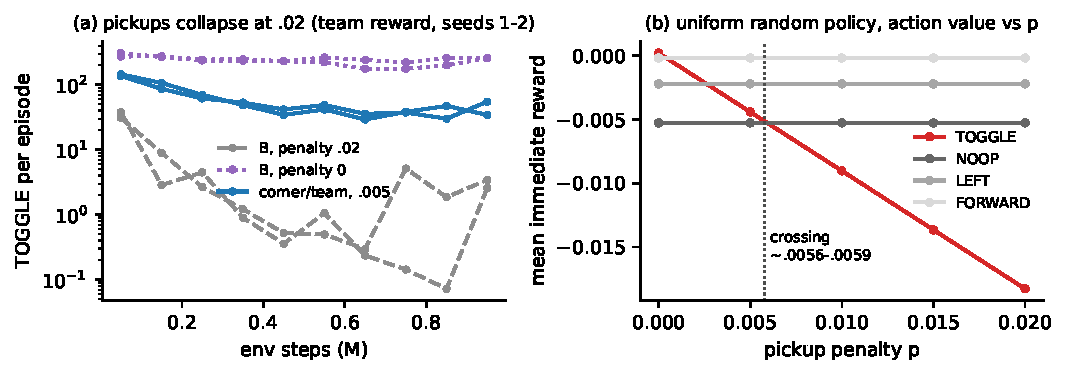
\includegraphics[width=\textwidth]{figures/fig_stall.pdf}
  \caption{(a) B 환경의 0.1M 구간별 TOGGLE/episode. 감점 .02에서는 0.1--0.2M에 붕괴하고, 0에서는 남발하며, .005는 그 사이에서 유지된다. (b) 무작위 정책에서 감점 $p$에 따른 행동별 평균 즉시 보상(A 환경, 학습 없음).}
  \label{fig:stall}
\end{figure}

\subsection{감점 .005에서의 1M 학습}
\label{sec:pen005}
감점 .005에서 1M 시점 학습 배송은 기존 .02의 5배 이상이었다(그림 \ref{fig:learning}a). 그러나 모든 run에서 0.6M 무렵부터 한 agent가 치고 나가 0.9M에는 배송의 82--99\%를 맡았고, 그 agent의 팀만 배송했다(그림 \ref{fig:learning}b, c).
독주 agent를 NOOP으로 두거나 먼 칸으로 옮겨도 나머지 agent는 거의 배송하지 않았다(그림 \ref{fig:removal}). 따라서 1M까지의 독주는 경쟁이나 통로 막힘이 아니라, 나머지가 아직 배우지 못한 결과다.
\easy{배송은 늘었지만 거의 한 로봇이 혼자 한다. 그 로봇을 치워도 다른 로봇은 일하지 않는다. 다른 로봇이 밀려난 게 아니라, 아직 일을 못 배운 것이다. 팀원의 critic을 나눠 주면 이들이 배우는지가 지금 진행 중인 실험의 질문이다.}
\detail{
  \item \textbf{조건 (E52)}: 기반 B(6 agent, 통신 3), 감점 .005, IPPO, seed 1·2, 1M. 모서리·팀과 모서리·개인 두 칸.
  \item \textbf{학습 (0.9--1M)}: 학습 배송/episode는 팀 1.17·1.01, 개인 1.16·1.35. 같은 seed의 기존 .02 B는 0.23·0.005였다. 평가 마지막 5회는 팀 0.81·0.38, 개인 0.99·0.83이다. 평가 배송이 3회 연속 1 이상이 된 것은 개인 s1(0.87M)뿐이다.
  \item \textbf{탐색}: 0.2M 이후 구간별 TOGGLE/episode 최저값은 팀 29--30, 개인 7--8이다. 요청되지 않은 선반 pickup은 팀 칸에서 약 23/episode로, 감점 0의 약 20\%다.
  \item \textbf{독주}: 최다 agent 비율은 팀 0.91·0.82, 개인 0.99·0.97이고, 독주 agent의 팀만 배송했다. 마지막 구간에서 잘못된 반납이 0.3--1.2/episode로 늘었다.
  \item \textbf{제거 진단 (E53)}: 정상 조건에서 독주 agent는 0.85--1.55/episode, 나머지 합은 0--0.15(확률적 정책)였다. 독주 agent를 NOOP으로 두거나 먼 칸으로 옮겨도 나머지는 0--0.3이었다. 결정적 평가에서는 모두 0이다. 요청 대기열은 팀별이라 다른 팀의 요청을 빼앗을 수 없다.
  \item \textbf{판정}: 사전 기준 다섯 가지 중 4번(배송 분산)만 실패했다.
  \item \textbf{근거}: EXPERIMENTS E52·E53, \texttt{output/pen005\_analysis\_20261023/}, \texttt{output/pilot\_verdicts/}.
}

\begin{figure}[t]
  \centering
  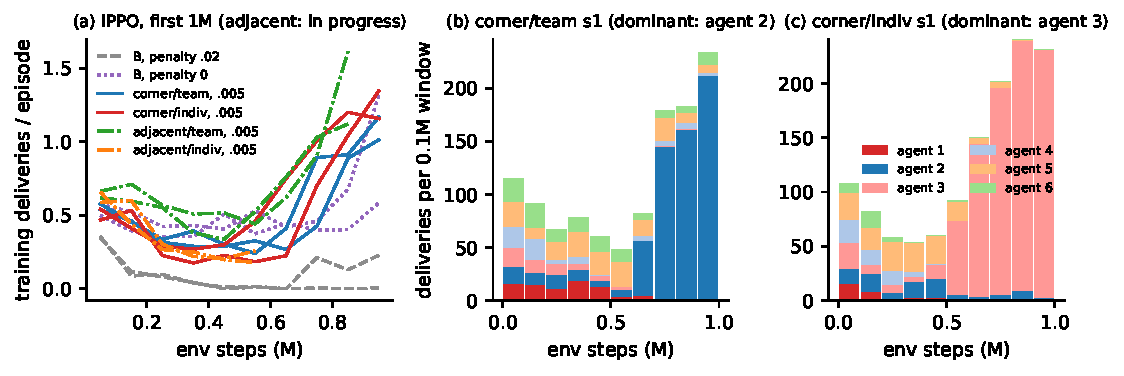
\includegraphics[width=\textwidth]{figures/fig_learning_1m.pdf}
  \caption{(a) IPPO 첫 1M의 학습 배송(seed 1·2). 인접 칸 두 개는 진행 중이다. (b, c) 0.1M 구간별 agent별 배송 수. 홀수 agent는 빨강 팀, 짝수 agent는 파랑 팀이다.}
  \label{fig:learning}
\end{figure}

\begin{figure}[t]
  \centering
  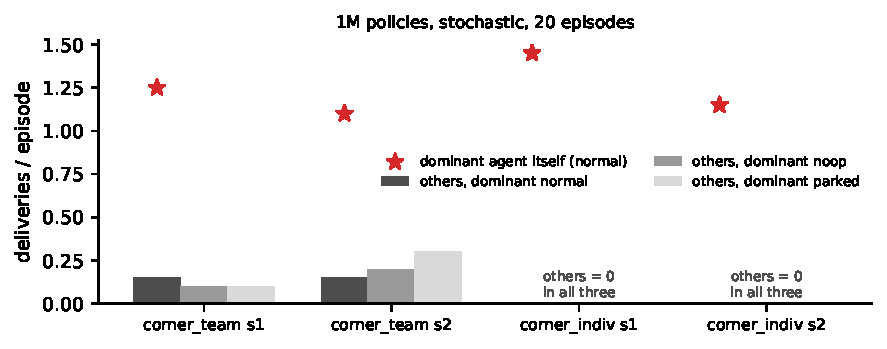
\includegraphics[width=0.75\textwidth]{figures/fig_removal.pdf}
  \caption{1M 정책에서 독주 agent를 제거했을 때 나머지 agent의 배송(확률적 정책, 20 episode). 별: 정상 조건에서 독주 agent 자신의 배송.}
  \label{fig:removal}
\end{figure}

\subsection{팀 식별: 보상 결합 대 정책 probe}
\label{sec:ident}
팀 보상 칸에서 보상 결합 probe는 네 checkpoint 모두 AUROC 1.00이었다. 정책 probe는 0.41--0.78이었다(그림 \ref{fig:ident}a).
온라인 판정(사건 1회로 판정)에서 팀 보상 칸은 대개 1.2만--3.6만 step 안에 15쌍을 모두 맞혔고 오답이 없었다.
개인 보상 칸에서는 보상 결합이 실패했을 뿐 아니라 15쌍 중 5--9쌍을 틀렸다(그림 \ref{fig:ident}b). 반응이 모두 0 근처라 거리가 작게 나오기 때문이며, 판정 보류 규칙이 필요하다.
\easy{팀 보상이면 ``저 칸에 배송이 일어났을 때 내가 상을 받는가''만 보면 팀이 바로 갈린다. 개인 보상이면 남의 배송으로 상을 받는 일이 없어서 이 방법이 통하지 않는다.}
\detail{
  \item \textbf{측정 조건}: 1M 이하 고정 정책으로 확률적 rollout 80 episode $\times$ 500 step을 돌렸다. 시야(Chebyshev $\le$ 5) 안에서 남이 일으킨 goal 배송만 셌다. 팀 필드는 판정에 쓰지 않았다.
  \item \textbf{B 팀, 감점 0 (E49)}: 보상 결합 AUROC는 네 checkpoint 모두 1.00(episode bootstrap 95\% 구간 1.00--1.00)이다. 정책 probe는 canonical .59--.78, v2 gate .41--.76, 방문 상태 .44--.78이었다.
  \item \textbf{모서리·팀 .005 (E52)}: 보상 결합 1.00, 정책 probe .46--.74. 모서리·개인 .005: 보상 결합 .38--.88, 정책 probe .43--.69.
  \item \textbf{식별 시점 (E50, E52)}: 사건 1회로 판정할 때 15쌍 모두 정답이 되기까지 B 감점 0에서 6,106--36,472 step, 모서리·팀에서 12,122--36,458 step이었다(s1 1M만 4만 step 안에 14/15). 오판정은 B 감점 0의 20개 조건 중 1회다. 모서리·개인에서는 4만 step 안에 15쌍 중 5--9쌍이 오판정이었다.
  \item \textbf{배운 agent 간 정책 probe (E53)}: 같은 goal 쌍과 다른 goal 쌍의 평균 JS는 v2 .095 대 .091, canonical .110--.111 대 .119--.121로, AUROC 0.56이었다. seed 계보에 따른 구조도 없었다(같은 run .149, 같은 seed .146, 다른 seed .141).
  \item \textbf{근거}: EXPERIMENTS E49·E50·E52·E53, \texttt{output/reward\_coupling\_20261022/}.
}

\begin{figure}[t]
  \centering
  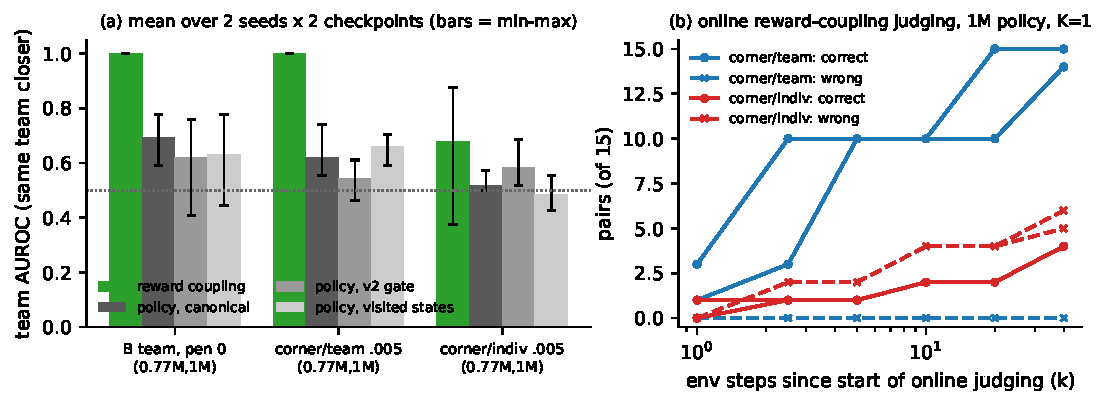
\includegraphics[width=\textwidth]{figures/fig_identification.pdf}
  \caption{(a) 팀 AUROC. 막대는 seed 2개 $\times$ checkpoint 2개(0.77M, 1M)의 평균, 오차 막대는 최소--최대다. (b) 1M 정책에서 보상 결합 probe로 온라인 판정한 정답(실선)과 오답(점선) 쌍 수.}
  \label{fig:ident}
\end{figure}

\paragraph{배운 agent끼리의 정책 probe.}
네 run의 독주 agent 4명(goal: (9,10) 3명, (0,10) 1명)을 같은 probe로 비교했다. 같은 goal 쌍과 다른 goal 쌍의 평균 JS는 v2 gate에서 0.095 대 0.091로 차이가 없었고, 가장 비슷한 쌍은 오히려 goal이 반대인 쌍이었다(그림 \ref{fig:probes} 아래 줄).
다만 이 agent들도 episode당 약 1회 배송하는 수준이라 충분히 학습된 정책이 아니다. 이 결과를 정책 probe의 구조적 실패로 결론 내리지 않는다.

\subsection{goal 방향 축으로 본 정책 probe}
\label{sec:axis}
\paragraph{무엇을 했나.} 먼저 gate probe 48개 가운데, 왼쪽 goal agent와 오른쪽 goal agent의 최적 첫 행동이 다른 probe를 지도에서 골랐다. 모서리 배치에서 13개, 인접 배치에서 3개다.
이 13개만으로 JS를 다시 재고, \ref{sec:axis-method}절의 goal 방향 축 $s_i$도 쟀다. 대상은 모서리 goal을 쓰는 기존 checkpoint 28개다(학습 없음).

\paragraph{결과.}
\begin{itemize}
  \item 13개만 써도 JS 팀 AUROC는 평균 0.49로, 48개 전부(0.51)보다 낫지 않았다.
  \item 그러나 $s_i$는 6-agent 칸 네 가지에서 자기 goal 쪽을 0.89--0.96의 AUROC로 가리켰다(그림 \ref{fig:axis}b). seed 1과 2는 goal 쪽이 서로 바뀌므로, agent 번호나 초기화가 만든 착시가 아니다.
  \item 쌍 단위로는 $|s_i - s_j|$의 AUROC가 0.70--0.73, 부호 규칙의 정확도가 0.76--0.83이었다(모서리·팀, 모서리·개인, 감점 0 칸). 같은 13개의 JS는 0.52--0.54였다(그림 \ref{fig:axis}c).
  \item 4-agent run(A, E1-F)에서는 나타나지 않았다. 이 run들은 1.5--2M에도 배송이 거의 없었다. 덜 학습된 탓일 수 있으나 확인하지 않았다.
\end{itemize}

\begin{figure}[t]
  \centering
  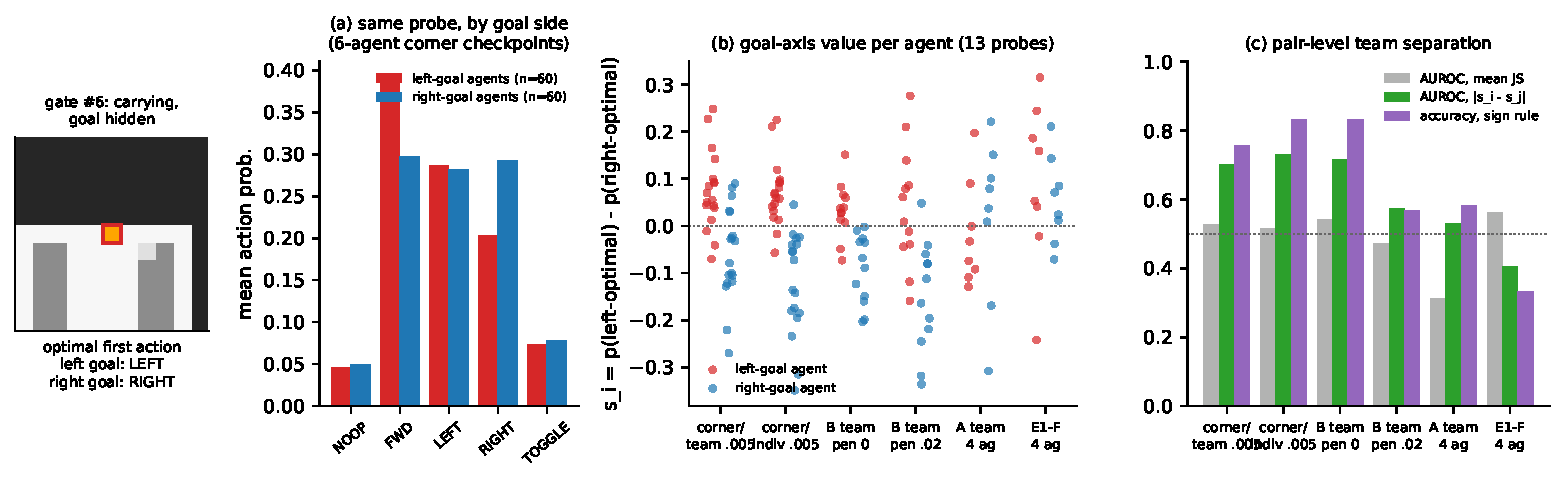
\includegraphics[width=\textwidth]{figures/fig_goal_axis.pdf}
  \caption{goal 방향 축. (a) goal 쪽에 따라 최적 행동이 다른 probe 하나와, 그 probe에서 왼쪽 goal agent·오른쪽 goal agent의 평균 행동 확률(6-agent 모서리 checkpoint의 모든 agent). (b) agent별 $s_i$. 빨강은 왼쪽 goal, 파랑은 오른쪽 goal agent다. (c) 쌍 단위 팀 구분: JS의 AUROC, $|s_i - s_j|$의 AUROC, 부호 규칙의 정확도(점선은 우연 수준).}
  \label{fig:axis}
\end{figure}

\easy{행동 확률 전체를 통째로 비교하면, 로봇마다 다른 사소한 버릇이 팀 차이를 가린다. 그래서 ``왼쪽 goal로 가는 행동을 더 고르나, 오른쪽 goal로 가는 행동을 더 고르나''만 따로 봤다. 그러자 목표가 다른 로봇끼리 확실히 달라졌다. 개인 보상이라 보상 결합이 통하지 않는 칸에서도 그렇다. 팀 쌍 6쌍 중 5쌍 정도를 맞히는 수준이라 아직 완벽하지는 않다.}
\detail{
  \item \textbf{판별 probe 선택}: E1-F v2 gate bank 48개에서 지도 BFS로 고른 13개 [1, 5, 6, 12, 15, 16, 23, 25, 27, 37, 41, 42, 47]. 운반 중에는 선반 칸에 들어갈 수 없다는 규칙을 썼다. 인접 goal에서는 3개뿐이다.
  \item \textbf{대상}: 모서리 goal checkpoint 28개(학습 없음, 가중치 hash 불변).
  \begin{itemize}[leftmargin=1.2em,itemsep=0pt,topsep=0pt]
    \item 모서리·팀 / 모서리·개인 .005: s1·s2 $\times$ 0.51/0.77/1M
    \item B 감점 0: s1·s2 $\times$ 0.77/1M
    \item B·A 감점 .02: s1·s2 $\times$ 1M/2M
    \item E1-F 1.54M: IPPO, PGCT, Oracle-team, All-peer
  \end{itemize}
  \item \textbf{JS}: 평균 팀 AUROC가 48개 .512, 13개 .493, 나머지 35개 .524였다. 13개가 나은 경우 6개, 나쁜 경우 12개다.
  \item \textbf{$s_i$가 자기 goal 쪽을 가리키는 AUROC}: 모서리·팀 .89, 모서리·개인 .96, B 감점 0 .89, B 감점 .02 .92, A .44, E1-F .56.
  \item \textbf{쌍 단위}: $|s_i - s_j|$ AUROC는 위 순서대로 .70 / .73 / .72 / .57 / .53 / .41. 같은 13개의 JS는 .53 / .52 / .54 / .47 / .31 / .56. 부호 규칙 정확도는 .76 / .83 / .83 / .57 / .58 / .33(같은 팀 유지 .72--.83, 다른 팀 거부 .78--.83, 6-agent 감점 .005·0 칸 기준). 28개 중 21개에서 축이 JS보다 높았다.
  \item \textbf{agent 단위}: 152명 전체에서 왼쪽·오른쪽 goal agent의 $s$ 분리 AUROC는 .74, 배운 agent 19명만 보면 .90이었다.
  \item \textbf{한계}: 6-agent는 seed 2개씩이고, 정책은 1M 이하(감점 .02는 2M)다. goal 후보 칸을 지도에서 안다고 가정하며, 두 goal 기준이다.
  \item \textbf{근거}: EXPERIMENTS E54, DECISIONS D80, \texttt{output/probe\_discriminative\_20261023/}.
}

\begin{figure}[t]
  \centering
  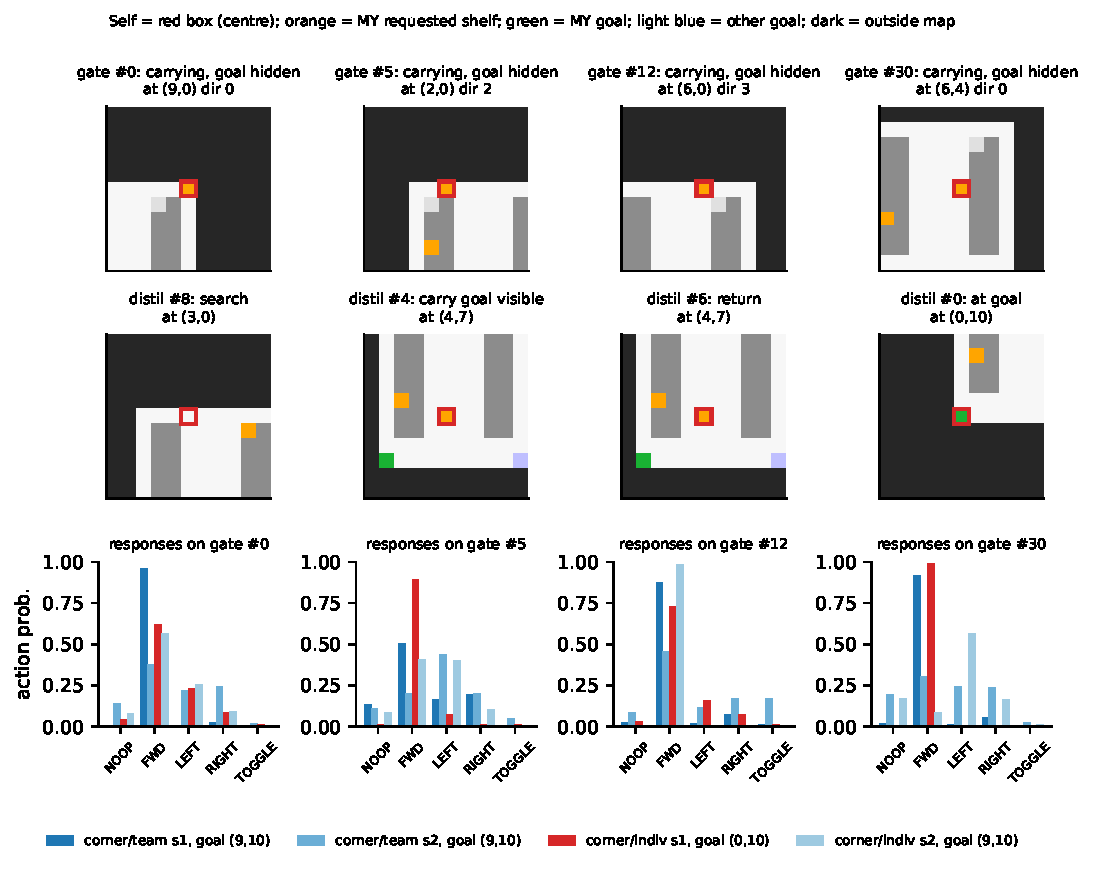
\includegraphics[width=\textwidth]{figures/fig_probes.pdf}
  \caption{probe 예시(E1-F 지도의 v2 bank). 위: gate probe(운반 중, goal 비가시). 가운데: 증류 probe(탐색, goal 가시 운반, 반납, goal 도착). 아래: 네 run의 1M 독주 agent가 gate probe에 낸 행동 분포. goal이 다른 agent(빨강)의 응답이 같은 goal agent들과 뚜렷이 다르지 않다.}
  \label{fig:probes}
\end{figure}

\subsection{독주 진단 정리와 해석의 한계}
\label{sec:limits}
기존 학습 경험상 센서 범위 5에서 어느 정도 배우는 데 2--5M이 걸렸고, 네 agent가 모두 배운 커리큘럼 모델은 8M에서 완성되었다. 1M은 학습 초입이다.
따라서 ``독주가 병목''이나 ``정책 probe는 구조적으로 실패''라는 결론은 보류한다. 보상 결합 결과는 배송 사건만 있으면 성립하므로 유지한다. goal 방향 축의 결과도 1M 이하의 정책에서 얻은 것이라, 더 학습된 정책에서는 더 뚜렷해지거나 달라질 수 있다.
\easy{1M은 학습 초입이다. 지금 보이는 ``한 명만 배운다''나 ``probe가 안 된다''는 학습이 덜 된 탓일 수 있다. 그래서 본 실험은 5M까지 본다.}
\detail{
  \item \textbf{학습 길이의 기준}: 이전 경험상 센서 범위 5에서 어느 정도 배우는 데 2--5M이 걸렸다. 네 agent가 모두 배운 커리큘럼 모델은 8M에 완성되었다. E1도 6.4M에서야 episode당 23--32회를 배송했다.
  \item \textbf{1M 결과의 위상}: 1M pilot은 초반 정체(0.1--0.2M)를 확인하려는 것이었다. 독주 agent도 1M에서 episode당 약 1회 배송하는 수준이다.
  \item \textbf{정정 (D78)}: ``독주가 핵심 병목''과 ``정책 probe 실패는 구조적''은 철회하거나 보류한다. 보상 결합 결과(E49·E50·E52)는 유지한다.
  \item \textbf{대응}: 메인 1단계 길이를 2M에서 5M으로 늘렸다. 2M·3M은 참고로만 보고, 판정은 5M에서 한다.
}

\FloatBarrier
%% ==================================================================
\section{진행 중인 실험}

\paragraph{메인 1단계 (Q2, 2026-10-23 시작).}
모서리·팀 칸(감점 .005)에서 IPPO, Oracle-team, All-peer를 seed 1--3, 각 5M step으로 돌린다(9 job, 동시 4개).
Oracle-team 대 IPPO는 ``팀원 critic을 받으면 배우는 agent가 늘어나는가''를 본다.
All-peer 대 Oracle-team에서 다른 팀 agent의 성적은 ``학습된 다른 팀 critic이 해로운가 이로운가''를 critic 품질의 교란 없이 잰다. 이 칸에는 이미 배운 donor가 있기 때문이다.
그림 \ref{fig:now-transfer}는 실제 상태에서 세 방법이 만드는 전이 그래프를, 그림 \ref{fig:now-probes}는 같은 칸에서 두 probe가 보는 것을 보여 준다.

\begin{figure}[t]
  \centering
  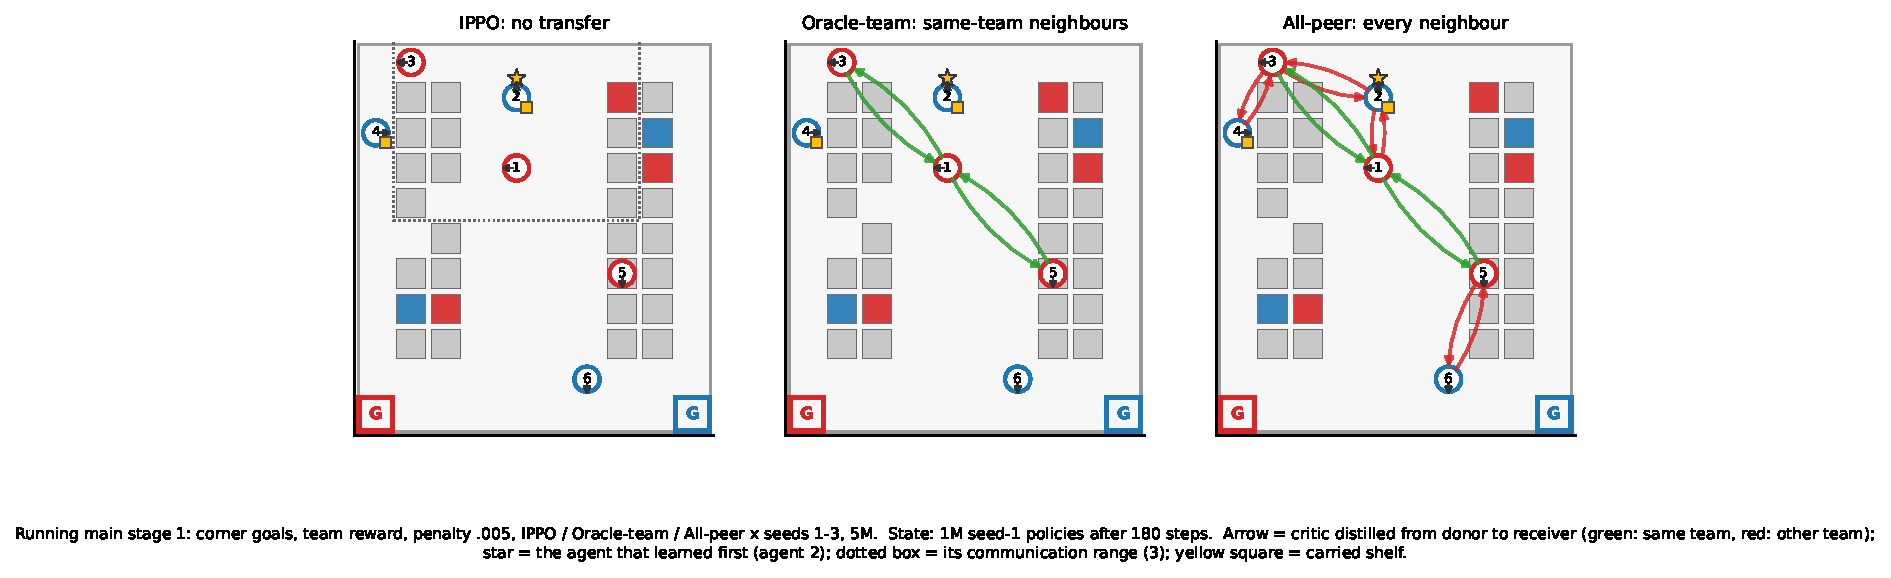
\includegraphics[width=\textwidth]{figures/fig_now_transfer.pdf}
  \caption{진행 중인 메인 1단계의 전이 그래프. 1M seed-1 정책으로 180 step 진행한 실제 상태다. 화살표는 donor에서 받는 쪽으로의 critic 증류(초록: 같은 팀, 빨강: 다른 팀), 별은 먼저 배운 agent 2, 점선 상자는 그 agent의 통신 범위(3), 노란 사각형은 운반 중인 선반이다.}
  \label{fig:now-transfer}
\end{figure}

\begin{figure}[t]
  \centering
  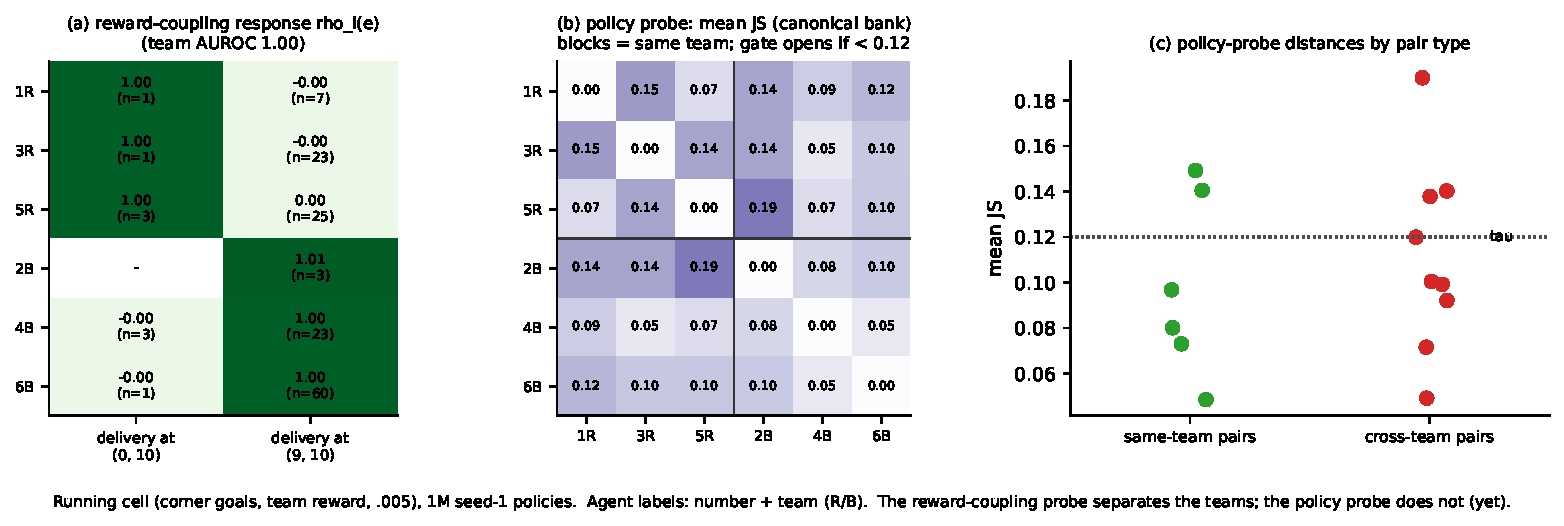
\includegraphics[width=\textwidth]{figures/fig_now_probes.pdf}
  \caption{진행 중인 칸(모서리·팀, .005)에서 두 probe가 보는 것(1M seed-1). (a) 보상 결합 반응 $\rho_i(e)$: 같은 팀은 같은 goal의 배송에 1, 다른 goal에 0으로 반응한다. (b) 정책 probe의 쌍별 평균 JS(canonical bank). 굵은 선으로 나눈 블록이 같은 팀이다. (c) 같은 팀 쌍과 다른 팀 쌍의 JS 분포. 두 분포가 겹쳐 gate가 팀을 가르지 못한다.}
  \label{fig:now-probes}
\end{figure}

\begin{table}[h]
\centering
\caption{메인 1단계의 사전 고정 기준(결과를 보기 전에 정함).}
\begin{tabularx}{\textwidth}{>{\raggedright\arraybackslash}p{4.2cm} L}
\toprule
항목 & 정의 \\
\midrule
배운 agent & 마지막 평가 5회(100 episode)에서 agent별 배송 $\ge 0.25$/episode \\
주 지표 & 배운 agent 수, 독주 agent를 뺀 배송 합, 팀별 배송, 독주 agent 자신의 배송, 다른 팀의 배송(All-peer 대 Oracle-team) \\
판정 시점 & 5M(2M·3M은 참고) \\
전이 효용 판정 & seed 3개 중 2개 이상에서 Oracle-team의 배운 agent 수가 IPPO보다 많음 \\
\bottomrule
\end{tabularx}
\end{table}

\detail{
  \item \textbf{대기열}: \texttt{latent\_team/run\_queue.ps1}, 이름 \texttt{queue\_20261023\_150050}, 2026-10-23 15:00 KST 시작. job 9개는 seed별로 IPPO, Oracle-team, All-peer 순서이며, 이 컴퓨터의 학습 프로세스가 4개 미만일 때만 다음 job을 띄운다.
  \item \textbf{환경}: \texttt{b\_e1f6\_comm3\_pen005}(6 agent 3+3, 센서 5, 통신 3, 팀 보상, 모서리 goal, 감점 .005). seed가 같으면 세 방법의 초기 가중치가 같다.
  \item \textbf{일정 (약 15 step/s 기준)}: 인접 칸이 끝나는 10-23 밤부터 시작해, 첫 4개는 10-27--28, 다음 4개는 11-01, 마지막 1개는 11-05 무렵 끝난다. 2M 중간 결과는 10-25 무렵 볼 수 있다.
  \item \textbf{2M 대신 5M}: 독주 agent의 배송 시작이 0.6--0.9M이고, 다른 agent는 2--5M에 배울 수 있어서다(\ref{sec:limits}절).
  \item \textbf{앱 밖 실행}: E1-F가 앱 업데이트로 멈춘 뒤로, 모든 학습은 Claude 앱 밖 PowerShell에서 돌린다.
}

\paragraph{2$\times$2 인접 칸 (IPPO 1M $\times$ seed 2).}
인접·팀과 인접·개인 칸이 진행 중이다. 초반 탐색이 되는지와 보상 결합으로 식별되는지를 본다.
정책 probe 판정에는 쓰지 않는다(1M이므로).

\FloatBarrier
%% ==================================================================
\section{향후 계획}

\begin{figure}[t]
  \centering
  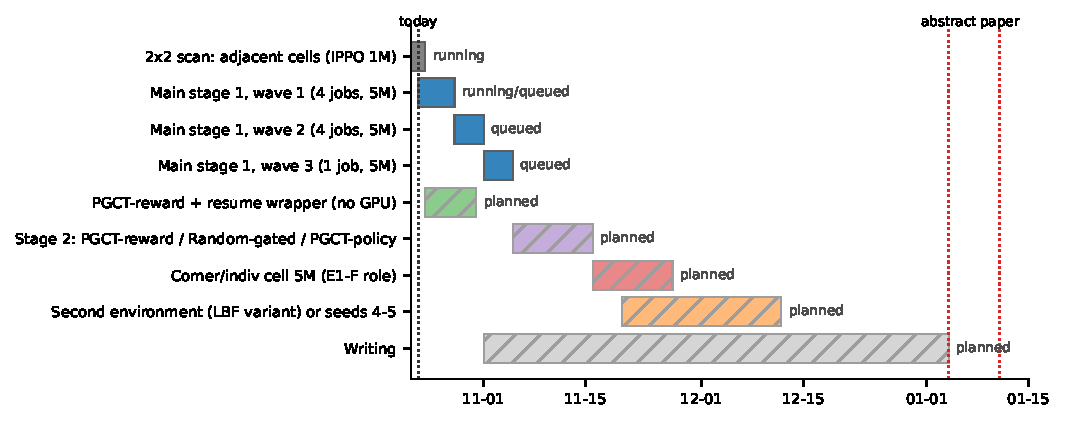
\includegraphics[width=\textwidth]{figures/fig_plan.pdf}
  \caption{2026-10-23 기준 일정. 실선은 실행 중이거나 대기열에 있고, 빗금은 계획이다. 5M job은 동시 4개일 때 약 4일 걸린다.}
  \label{fig:plan}
\end{figure}

\begin{enumerate}
  \item \textbf{1단계를 기다리는 동안 (GPU 없이)}: 인접 칸 분석(goal 방향 축이 인접 배치에서 실패하는지 포함), PGCT-reward와 PGCT-축 구현(판정 보류 규칙 포함, trainer 변경 없음), 부호 규칙과 EMA를 묶은 시점별 정확도, 판별 probe를 더 많이 만들었을 때의 효과, optimizer까지 복원하는 이어 학습 wrapper, 결과와 무관한 원고.
  \item \textbf{11월 초 분기}:
  \begin{itemize}
    \item Oracle-team이 배운 agent를 늘리면: 같은 칸에서 PGCT-reward, PGCT-축(goal 방향 축 gate), Random-gated를 seed 3개, 5M으로 돌리고, 여러 agent가 배운 Oracle-team checkpoint로 정책 probe를 다시 시험한다. JS 기반 PGCT-정책은 비교용으로만 둔다.
    \item 늘리지 못하면: 탐색(entropy, 감점 일정)을 진단하고, 원고의 무게를 식별 가능성 분석으로 옮긴다.
  \end{itemize}
  \item \textbf{11월 중순--12월 초}: 모서리·개인 칸 5M(E1-F의 역할, 정책 probe가 꼭 필요한 칸), 그리고 두 번째 환경 또는 seed 4·5.
  \item \textbf{두 번째 환경}: SMAC은 학습자 사이에 잠재 팀이 없고, Hide-and-Seek은 팀이 곧 역할이며 자기 편을 안다. 두 팀이 서로 다른 먹이를 모으는 Level-Based Foraging 변형을 1순위로, 팀별 랜드마크를 둔 MPE 변형을 차선으로 둔다.
  \item \textbf{12월 중순 이후}: 원고 마무리. IJCAI 2027 초록 마감 1월 4일, 본문 1월 11일(AoE).
\end{enumerate}

\paragraph{2단계에서 비교할 gate.}
그림 \ref{fig:next-gates}는 같은 상태에서 세 gate가 고를 donor를 보여 준다. 보상 결합 gate는 같은 팀 연결만 만들고, 정책 gate는 다른 팀 연결이 더 많으며, Random-gated는 정책 gate와 같은 수의 연결을 무작위로 고른다.

\begin{figure}[t]
  \centering
  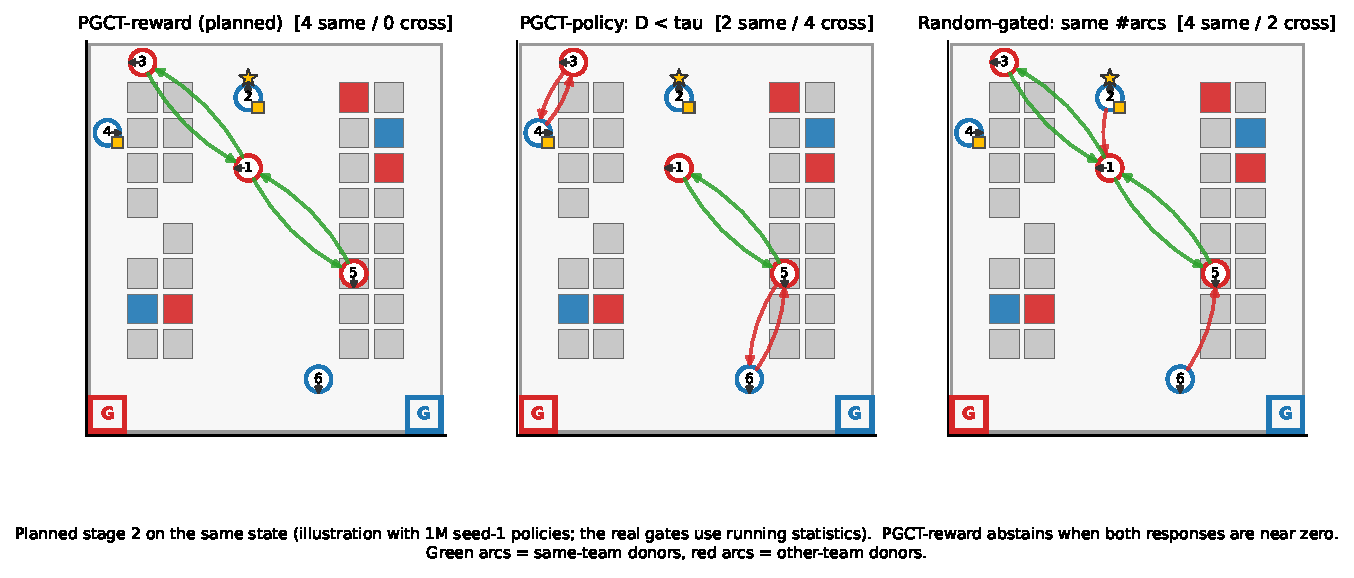
\includegraphics[width=\textwidth]{figures/fig_next_gates.pdf}
  \caption{계획된 2단계의 gate 비교(그림 \ref{fig:now-transfer}와 같은 상태, 1M seed-1 정책으로 만든 예시). 실제 gate는 학습 중 누적 통계를 쓴다. PGCT-reward는 두 agent의 반응이 모두 0 근처면 판정을 보류한다. 제목의 괄호는 같은 팀 / 다른 팀 연결 수다.}
  \label{fig:next-gates}
\end{figure}

\paragraph{모서리·개인 칸에서의 정책 probe.}
정책 probe가 팀을 가를 수 있으려면, goal이 보이지 않는 운반 상태에서 최적 행동이 goal 쪽에 따라 달라야 한다(조건 (가)).
지도에서 너비 우선 탐색으로 최단 경로의 첫 행동을 계산하면, v2 gate probe 48개 가운데 모서리 goal에서는 13개, 인접 goal에서는 3개만 왼쪽 goal과 오른쪽 goal의 최적 첫 행동이 겹치지 않는다(그림 \ref{fig:next-probes}).
즉 모서리 배치에서도 gate probe의 약 1/4만 원리상 팀을 가를 수 있다. 충분히 학습된 정책이 이 probe들에서 실제로 다르게 답하는지가 5M 실험에서 볼 핵심이다.

\begin{figure}[t]
  \centering
  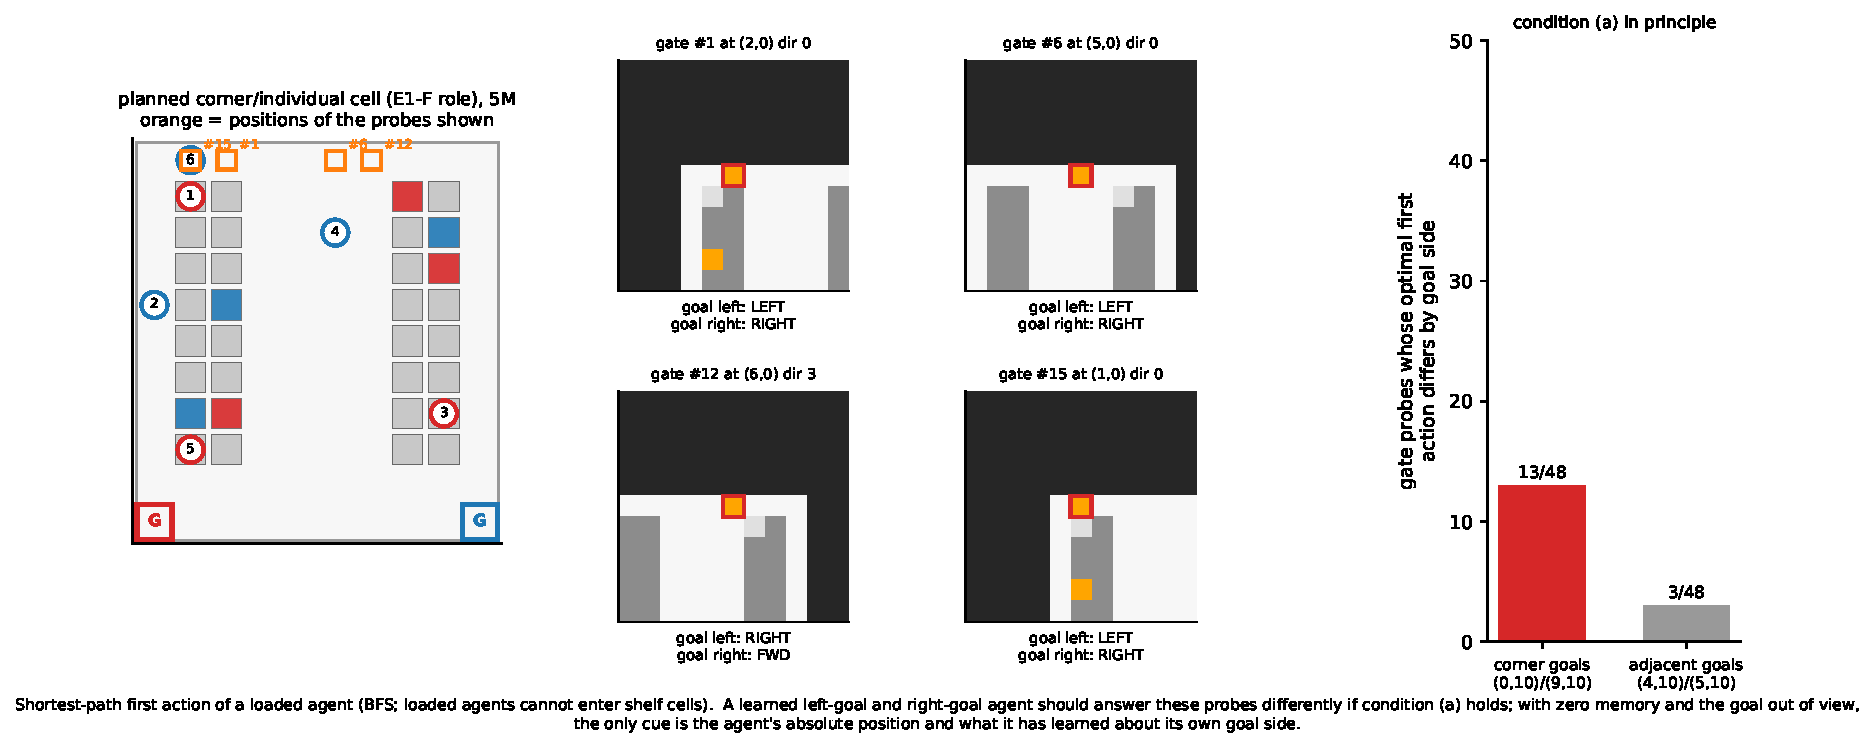
\includegraphics[width=\textwidth]{figures/fig_next_probes.pdf}
  \caption{계획된 모서리·개인 칸(E1-F 역할). 왼쪽: 지도와 예시 probe의 위치. 가운데: 왼쪽 goal agent와 오른쪽 goal agent의 최적 첫 행동이 다른 gate probe 예시. 오른쪽: 두 goal 배치에서 이런 probe의 수(너비 우선 탐색, 운반 중에는 선반 칸에 들어갈 수 없음).}
  \label{fig:next-probes}
\end{figure}

\paragraph{두 번째 환경(개념).}
그림 \ref{fig:next-lbf}는 두 팀이 서로 다른 종류의 먹이를 모으는 Level-Based Foraging 변형의 개념도다. 아직 구현하지 않았다. 먹이 배치(섞임/팀별 구역)와 보상 방식을 바꾸면 RWARE와 같은 2$\times$2를 만들 수 있다.

\begin{figure}[t]
  \centering
  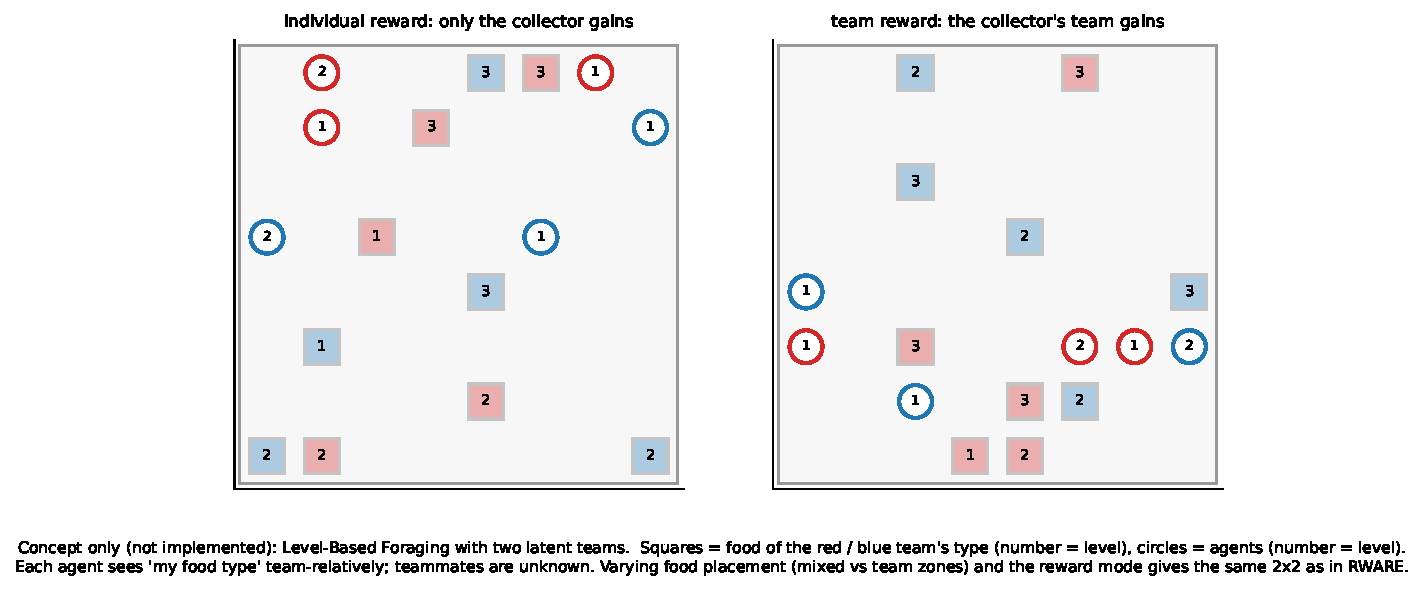
\includegraphics[width=0.85\textwidth]{figures/fig_next_lbf.pdf}
  \caption{두 번째 환경 후보의 개념도(구현 전). 사각형은 빨강·파랑 팀 종류의 먹이(숫자는 레벨), 원은 agent(숫자는 레벨)다. agent는 ``내 먹이 종류''를 팀 기준으로 보고, 팀원은 모른다.}
  \label{fig:next-lbf}
\end{figure}

\FloatBarrier
%% ==================================================================
\section{논의}

\paragraph{범위.}
보상 결합만으로는 ``공유 보상에서 팀원 찾기''로 범위가 좁아지고, 팀 보상에서는 사실상 팀의 정의라 자명하다는 비판을 받기 쉽다.
goal 방향 축은 개인 보상 칸(조건 (가)만 있는 칸)에서 처음으로 쓸 만한 신호를 보였다. 이 결과가 더 학습된 정책과 더 많은 seed에서 유지되면, 논문은 ``팀 보상에서는 보상 결합, 개인 보상에서는 goal 방향 축''이라는 조건별 식별로 범위를 넓힐 수 있다.

\paragraph{goal 방향 축의 가정.}
goal 후보 칸이 지도의 어디인지 안다고 가정한다(지도에 보이므로 라벨은 아니다). 축은 goal 쌍마다 정의되므로 팀이 셋 이상이면 여러 축이 필요하다. 인접 배치처럼 판별 probe가 거의 없으면(3개) 작동하지 않을 것으로 예상한다.

\paragraph{가정 줄이기.}
``같은 목표면 비슷하게 행동한다''는 전제가 아니라 조건 (가)로 낮춘다. 명제 1·2는 부록으로 옮기고, 고정 $\tau$ 대신 이웃 간 상대 순위 판정을 검증한다. 남는 핵심 가정은 probe 비교 가능성과 공통 probe 생성 규칙이다.

\paragraph{교란 요인.}
(1) seed 하나의 성능 비교는 발견 운이 증폭된 값일 수 있다. (2) 조건마다 기반 설정이 달랐던 비교는 2$\times$2로 대체했다. (3) 다른 팀 critic의 해악은 donor가 학습된 조건에서만 잴 수 있다.

%% ==================================================================
\section{결론}
PGCT의 JS 기반 정책 probe gate는 지금까지 팀을 안정적으로 가르지 못했다. 그 과정에서 환경의 선반 집기 정체를 찾아 감점 .005로 풀었다.
팀 보상에서는 보상 결합 probe가 팀을 빠르고 정확하게 찾고, 개인 보상에서도 정책 응답을 goal 방향 축으로 보면 팀 쌍의 약 80\%를 가를 수 있다는 첫 증거를 얻었다.
이제 남은 핵심 질문은 두 가지다. 팀원 critic 전이가 실제로 학습을 돕는가(진행 중, 5M). 그리고 goal 방향 축이 더 학습된 정책과 학습 중 gate에서도 유지되는가(계획).

%% ==================================================================
\begin{thebibliography}{99}
\bibitem{christianos2020} F. Christianos, L. Sch\"afer, S. V. Albrecht. Shared experience actor-critic for multi-agent reinforcement learning. NeurIPS, 2020.
\bibitem{christianos2021} F. Christianos, G. Papoudakis, A. Rahman, S. V. Albrecht. Scaling multi-agent reinforcement learning with selective parameter sharing. ICML, 2021.
\bibitem{derstroff2024} C. Derstroff, M. Cerrato, J. Brugger, J. Peters, S. Kramer. Peer learning: Learning complex policies in groups from scratch via action recommendations. AAAI, 2024.
\bibitem{du2025} H. Du, H. Nguyen, S. Thudumu, R. Vasa, K. Mouzakis. Goal-oriented multi-agent reinforcement learning for decentralized agent teams. arXiv:2511.11992, 2025.
\bibitem{hu2024} T. Hu, Z. Pu, X. Ai, T. Qiu, J. Yi. Measuring policy distance for multi-agent reinforcement learning. AAMAS, 2024.
\bibitem{idrl} Classifying ambiguous identities in hidden-role stochastic games with multi-agent reinforcement learning (IDRL). arXiv:2210.12896.
\bibitem{papoudakis2021} G. Papoudakis, F. Christianos, L. Sch\"afer, S. V. Albrecht. Benchmarking multi-agent deep reinforcement learning algorithms in cooperative tasks. NeurIPS Datasets and Benchmarks, 2021.
\bibitem{rusu2016} A. A. Rusu et al. Policy distillation. ICLR, 2016.
\bibitem{schulman2017} J. Schulman, F. Wolski, P. Dhariwal, A. Radford, O. Klimov. Proximal policy optimization algorithms. arXiv:1707.06347, 2017.
\bibitem{zhang2018} K. Zhang, Z. Yang, H. Liu, T. Zhang, T. Ba\c{s}ar. Fully decentralized multi-agent reinforcement learning with networked agents. ICML, 2018.
\end{thebibliography}

\appendix
\section{실험별 세부 요약}
모든 실험은 IPPO 계열 순환 PPO 학습기(semantic CNN, 128 unit GRU)를 쓴다. 평가는 결정적 정책 20 episode $\times$ 500 step이다. ``학습 없음''은 고정 checkpoint나 무작위 정책만 썼다는 뜻이다.

{\small
\begin{xltabular}{\textwidth}{>{\raggedright\arraybackslash}p{1.5cm} >{\raggedright\arraybackslash}p{4.4cm} >{\raggedright\arraybackslash}p{1.7cm} L}
\toprule
기록 & 조건 & 상태 & 핵심 수치 \\
\midrule
\endhead
E24, E27 & E1: 4 agent, 개인 보상, goal 인접, 통신 5, 감점 .02, 다섯 방법, seed 1 & 6.4M 완료 & 최종 IPPO 23.2, All-peer 19.4, PGCT 27.3, Oracle-team 32.2. 같은 팀 probe 거리 .333 > 다른 팀 .276 \\
E26, E28 & E1-F: E1에서 goal만 모서리, 다섯 방법, seed 1 & 1.536M 중단 & 평가 배송 거의 0. gate가 같은 팀을 고르지 않음 \\
E29--E34 & 고정 checkpoint의 정책 probe 점검 & 학습 없음 & 자기 표류 $\approx$ 팀 차이. 계보 간 재현 실패 \\
E35 & Random-gated 구현 & smoke & PGCT 실측 연결 수에 맞춤 \\
E36--E39 & 보상 probe $\hat r(o,a)$, 궤적 probe & 학습 없음 & 인위적 상태 AUROC .38--.62(팀별 보상이 다른 query 2\%). 실제 운반 창 Q\_diff .67--.79 \\
E40--E43 & 후보 A(4 agent, 통신 5)·B(6 agent, 통신 3), 팀 보상, 감점 .02, IPPO seed 1·2 & 2M 완료 & A s2 1.89M, B s1 1.13M에 각각 한 agent만 배움. 나머지는 배송 없음 \\
E44 & 무작위 정책 행동별 즉시 보상(A) & 학습 없음 & TOGGLE $-0.0183$로 최저, TOGGLE의 93\%가 감점 \\
E45, E46 & A·B 감점 0, IPPO seed 1·2 & 1M 완료 & TOGGLE 100--300/ep 유지, 요청되지 않은 pickup 50--150/ep, 평가 onset 없음 \\
E47 & 감점 0--.02 sweep(무작위 정책) & 학습 없음 & TOGGLE $\approx 0.0002 - 0.93p$, 교차 $p \approx$ .0056--.0059 \\
E48, E52 & 모서리·팀(B) 감점 .005, IPPO seed 1·2 & 1M 완료 & 학습 배송 1.17·1.01/ep, 최다 agent 0.91·0.82, 판정 4번만 실패 \\
E51, E52 & 모서리·개인(B 기반) 감점 .005, IPPO seed 1·2 & 1M 완료 & 학습 배송 1.16·1.35/ep, 평가 onset s1 0.87M, 최다 agent 0.99·0.97 \\
E51 & 인접·팀, 인접·개인(B 기반) 감점 .005, IPPO seed 1·2 & 진행 중 & 10-23 17시 기준 약 0.82M, 0.55M \\
E49 & B 감점 0의 보상 결합 대 정책 probe & 학습 없음 & 보상 결합 1.00, 정책 .41--.78 \\
E50 & 보상 결합 온라인 식별 시점 & 학습 없음 & 15쌍 정답까지 6,106--36,472 step(사건 1회), 오판정 1/20 \\
E53 & 독주 agent 제거 평가, 배운 agent 간 정책 probe & 학습 없음 & 제거 후 나머지 0--0.3/ep. 같은·다른 goal JS .095·.091 \\
E54 & 판별 probe 13개, goal 방향 축 & 학습 없음 & JS 13개 .493. 축 방향 AUROC .89--.96(6 agent). 부호 규칙 .76--.83 \\
메인 1단계 & 모서리·팀 감점 .005, IPPO·Oracle-team·All-peer $\times$ seed 1--3 & 5M, 진행 중 & 10-23 15:00 대기열 시작, 11월 초 종료 예상 \\
\bottomrule
\end{xltabular}
}

\section{기록 번호와 근거 파일}
수치의 근거는 저장소의 \texttt{EXPERIMENTS.md}(E), \texttt{DECISIONS.md}(D), \texttt{EXPERIMENT\_STORY.md}와 아래 파일이다.
\begin{center}
\begin{tabularx}{\textwidth}{>{\raggedright\arraybackslash}p{2.6cm} L L}
\toprule
기록 & 내용 & 파일 \\
\midrule
E24, E27 & E1 처음부터 학습 & \texttt{output/paper\_e1\_20261018/} \\
E29--E39 & probe 점검, 보상 probe & \texttt{output/probe\_*\_20261019/}, \texttt{output/reward\_probe\_20261019/} \\
E43, E44 & 후보 pilot, 선반 집기 정체 & \texttt{output/pickup\_stall\_20261021/} \\
E46--E48 & 감점 조정 & \texttt{output/nopen\_pilot\_20261022/}, \texttt{output/penalty\_sweep\_20261022/} \\
E49, E50 & 보상 결합, 식별 시점 & \texttt{output/reward\_coupling\_20261022/} \\
E51--E53 & 2$\times$2, pen005 분석, 독주 진단 & \texttt{output/pen005\_analysis\_20261023/}, \texttt{output/pilot\_verdicts/} \\
E54 & 판별 probe 13개, goal 방향 축 & \texttt{output/probe\_discriminative\_20261023/} \\
D71--D80 & 독창성 재점검, 해석 정정, 계획, goal 방향 축 & \texttt{DECISIONS.md} \\
그림 & 이 문서의 그림 전부 & \texttt{output/pgct\_progress\_paper\_20261023/make\_figures.py} \\
\bottomrule
\end{tabularx}
\end{center}

\end{document}
